A análise de sentimento é uma técnica de processamento de linguagem natural que envolve a identificação e extração de informações subjetivas a partir de dados textuais. Esse processo pode ser usado para identificar a polaridade, ou tom emocional, de um determinado texto, o que pode ser útil em várias aplicações, como pesquisa de mercado e análise de mídias sociais \cite{2008_Pang}. Pesquisas anteriores demonstraram a utilidade da análise de sentimento em diversos domínios, incluindo política, negócios e saúde \cite{2016_Chen_IP}.

Técnicas de aprendizado de máquina podem ser usadas para automatizar o processo de análise de sentimento. Essas técnicas envolvem o treinamento de um modelo de aprendizado de máquina em um conjunto de dados rotulados, onde os rótulos indicam a polaridade dos dados textuais. Uma vez treinado, o modelo pode ser usado para prever a polaridade de novos dados textuais que não foram vistos anteriormente. Algoritmos de aprendizado de máquina comumente usados para análise de sentimento incluem regressão logística, máquinas de vetor de suporte e redes neurais \cite{2013_Haddi}.

\section{Processamento de linguagem natural e Análise de sentimento}

A análise de sentimento é uma técnica de processamento de linguagem natural amplamente utilizada para identificar e extrair informações subjetivas de dados textuais. Essa abordagem envolve a identificação da polaridade ou tom emocional presente em um determinado texto \cite{2008_Pang}, o que pode ser aplicado em diversas áreas, como pesquisa de mercado e análise de mídias sociais \cite{2015_Nguyen}.

Técnicas de aprendizado de máquina, como o uso do Natural Language Toolkit (NLTK), são frequentemente empregadas para automatizar o processo de análise de sentimento. O NLTK é uma biblioteca em Python que fornece uma ampla gama de ferramentas e recursos para tarefas de processamento de linguagem natural, incluindo a análise de sentimentos \cite{2009_Bird_BOOK}. Ele oferece uma variedade de recursos, como classificadores pré-treinados, dicionários léxicos, algoritmos de tokenização e técnicas de stemming.

Para realizar a análise de sentimento, o NLTK oferece acesso a dicionários léxicos, que são conjuntos de palavras pré-definidas associadas a uma polaridade de sentimento (positiva, negativa ou neutra). Esses dicionários podem ser usados para atribuir uma polaridade a palavras individuais em um texto e calcular a polaridade geral do texto com base nessas palavras \cite{2012_Souza_IP}. Além disso, o NLTK também suporta técnicas mais avançadas, como a análise sintática e a detecção de sarcasmo, que podem aprimorar a precisão da análise de sentimento \cite{2014_Hutto}.

A análise de sentimento com o uso do NLTK geralmente segue um processo que envolve o pré-processamento dos textos, a tokenização (divisão em palavras ou frases), a atribuição de polaridade a cada palavra com base no dicionário léxico e o cálculo de uma pontuação geral de sentimento para o texto \cite{2013_Haddi}. Essa pontuação pode ser usada para classificar o texto como positivo, negativo ou neutro.

Além disso, o NLTK oferece recursos adicionais para aprimorar a análise de sentimento, como a remoção de stop words (palavras comuns que geralmente não carregam um significado emocional) e a lematização (redução de palavras a sua forma básica, por exemplo, reduzir 'correndo' a 'correr').

Ao combinar as técnicas oferecidas pelo NLTK com algoritmos de aprendizado de máquina, como regressão logística, máquinas de vetor de suporte e redes neurais, é possível obter modelos de análise de sentimento mais sofisticados e precisos \cite{2014_Kim}.

No contexto específico do Colab, a análise de sentimento pode desempenhar um papel fundamental na detecção e mitigação da formação de câmaras de eco. Pesquisas anteriores têm demonstrado que a análise de sentimento pode ser utilizada para identificar as crenças e inclinações políticas dos usuários com base em sua linguagem e sentimentos expressos nas postagens de mídias sociais. Algoritmos de aprendizado de máquina, como Naive Bayes, Random Forest e Support Vector Machines (SVM), têm sido amplamente aplicados na análise de sentimento nesse contexto como por exemplo demonstrado em \citeonline{2014_Hutto}.

Para identificar câmaras de eco, a análise de sentimento pode ser usada como uma métrica para medir a homofilia em uma rede social. A homofilia se refere à tendência dos indivíduos de se associarem com outros que são semelhantes a eles em termos de características, opiniões e sentimentos. Ao analisar o sentimento expresso nas postagens dos usuários, podemos determinar se um grupo de usuários está polarizado, ou seja, se a maioria de suas postagens apresenta um sentimento ou inclinação política semelhante.

Além de identificar a polarização, a análise de sentimento também pode revelar os tópicos específicos que estão impulsionando a polarização dentro dessas câmaras de eco. Ao examinar o conteúdo das postagens e identificar os principais temas discutidos, é possível compreender melhor os fatores que contribuem para a formação e manutenção dessas câmaras de eco.

No contexto do Colab, este estudo propõe a introdução de duas métricas adicionais no modelo de dados dos usuários: score e persona. O score refere-se à classificação das postagens como positivas ou negativas, com base em dicionários léxicos. Essa abordagem tem sido aplicada em diversos domínios de negócios e sociais, uma vez que as opiniões desempenham um papel central em nossas atividades diárias e influenciam nossos comportamentos \cite{2012_Souza_IP}.

As personas, por sua vez, são representações fictícias e generalizadas de grupos de usuários que compartilham características e comportamentos semelhantes. No contexto do Colab, duas personas principais foram identificadas: os 'Helpers' e os 'Complainers'. Os Helpers são caracterizados por um comportamento proativo e colaborativo, envolvendo-se em atividades de ajuda e compartilhamento de informações úteis. Por outro lado, os Complainers têm um comportamento mais crítico ou negativo, expressando insatisfação ou críticas.

Durante o estudo, foram aplicadas técnicas avançadas de análise de sentimento para identificar as personas "Helpers" e "Complainers" dentro do Colab, com base nos padrões de linguagem e sentimentos expressos nas postagens dos usuários. Essas personas desempenharam papéis distintos na comunidade do Colab, contribuindo para a colaboração e o aprimoramento contínuo da plataforma. Em um mundo ideal, usuários com essas personas coexistiriam em harmonia, compartilhando informações e opiniões de maneira construtiva. No entanto, em muitos casos, essas personas podem se tornar polarizadas, reforçando suas crenças e limitando a diversidade de perspectivas. Essa polarização pode levar à formação de câmaras de eco, onde os usuários são expostos principalmente a informações e opiniões que confirmam suas crenças existentes, pois interagem primariamente com outros usuários que se encaixam na mesma persona. Ao realizar analises de sentimento e classificar usuários em personas baseadas em suas postagens, ganhamos insights sobre como esses usuários se distribuem na rede, identificando padrões que podem indicar os fatores que influenciam a formação dessas bolhas. Existem de fato bolhas de personas de usuários na rede do Colab? Se existem, será que se trata de um comportamento dos usuários ou as plataformas de mídias sociais, através de um viés algorítimico, têm um papel ativo na formação dessas bolhas? Quais ações o Colab pode tomar para mitigar esses efeitos negativos e promover um discurso mais distribuído e menos polarizado? Essas são algumas das questões que pretendemos responder incorporando métricas provenientes de análise de sentimento no modelo de dados dos usuários.

\subsection*{Análise de Sentimento, homofilia e polarização}

No contexto da polarização em redes sociais, a Análise de Sentimento é uma ferramenta poderosa para detectar e mitigar a formação de câmaras de eco. Pesquisas anteriores mostraram que a análise de sentimento pode ser usada para identificar as crenças e inclinações políticas dos usuários com base em sua linguagem e sentimento expressos em postagens de mídias sociais. Algoritmos de aprendizado de máquina, como Naive Bayes, Random Forest e Support Vector Machines (SVM), têm sido amplamente utilizados para análise de sentimento \cite{2014_Hutto}.

Para identificar câmaras de eco, a análise de sentimento pode ser usada como uma métrica para medir a homofilia em uma rede social. A homofilia refere-se à tendência dos indivíduos de se associarem com outros que são semelhantes a eles em termos de características, opiniões e sentimentos. Ao analisar o sentimento expresso nas postagens de usuários, podemos determinar se um grupo de usuários está polarizado, ou seja, se a maioria de suas postagens apresenta um sentimento ou inclinação política semelhante.

A análise de sentimento permite medir o grau de polarização dentro desse grupo, fornecendo uma medida quantitativa do nível de homofilia na rede. Se os usuários dentro de um grupo apresentarem predominantemente sentimentos semelhantes, isso indica uma maior homofilia e uma maior probabilidade de formação de uma câmara de eco.

Além de identificar a polarização, a análise de sentimento também pode revelar os tópicos específicos que estão impulsionando a polarização dentro dessas câmaras de eco. Ao examinar o conteúdo das postagens e identificar os principais temas discutidos, é possível compreender melhor os fatores que contribuem para a formação e manutenção dessas câmaras de eco.

Com essa abordagem, a análise de sentimento não apenas fornece insights sobre a polarização em uma rede social, mas também ajuda a identificar os grupos de usuários que estão mais propensos a formar câmaras de eco e a perpetuar a polarização. Essas informações são valiosas para a compreensão dos padrões de interação e para o desenvolvimento de estratégias de mitigação da polarização e promoção do diálogo diversificado e inclusivo.

Por exemplo, em um estudo de \citeonline{2014_Colleoni}, a análise de sentimento foi usada para medir a polarização de usuários em discussões políticas no Twitter. Os autores descobriram que os usuários tendem a se agrupar em torno de indivíduos com opiniões semelhantes e que esse agrupamento leva à formação de câmaras de eco. Os autores sugeriram que a análise de sentimento poderia ser usada para identificar os usuários que estão impulsionando a polarização e direcioná-los com contra-argumentos ou pontos de vista alternativos.

\section{Personas e Scores: Novas Métricas para Análise de Sentimento das Postagens do Colab}

Nesse capitulo, realizamos alguns experimentos utilizando Analise de Sentimento no conteúdo das postagens dos usuários do Colab. O objetivo deste experimento é criar duas métricas adicionais no modelo de dados dos usuários do Colab: score e persona. O score se refere à classificação das postagens do usuário como positiva ou negativa de acordo com os dicionários léxicos. A classificação de persona envolve o usuário ser classificado como "helper" ou "complainer" de acordo com critérios específicos.

\subsection*{Score}
O score é uma métrica que classifica as postagens do usuário como positivas ou negativas. Esta classificação é baseada em dicionários léxicos, que são conjuntos de palavras pré-definidas associadas a uma polaridade de sentimento (positiva, negativa ou neutra). A análise de sentimento tem sido aplicada em quase todos os domínios de negócios e sociais, pois as opiniões são centrais para quase todas as atividades humanas e são influenciadores-chave de nossos comportamentos.

\subsection*{Personas}

Personas são representações fictícias e generalizadas de um grupo de usuários que compartilham características e comportamentos semelhantes. No contexto das redes sociais, as personas representam os diferentes tipos de usuários que interagem dentro dessas plataformas. Essas personas podem ser identificadas e categorizadas com base em uma variedade de fatores, incluindo, entre outros, seus comportamentos online, interesses, padrões de comunicação e atividades de postagem.

No contexto do Colab, propomos a hipótese de duas personas principais: os "Helpers" e os "Complainers". Essas personas são identificadas com base em suas atividades de postagem e interações dentro da plataforma.

\subsubsection*{Helpers}

A persona "helper" é caracterizada por um comportamento proativo e colaborativo em uma comunidade online. Esses indivíduos são frequentemente encontrados respondendo a perguntas, oferecendo conselhos e compartilhando informações úteis com outros membros da comunidade. Eles tendem a expressar sentimentos positivos em suas postagens e são motivados pelo desejo de ajudar os outros e contribuir para a comunidade.

Os "helpers" são fundamentais para o sucesso de qualquer comunidade online, pois eles ajudam a criar um ambiente de apoio e colaboração. Eles são frequentemente vistos como líderes informais ou especialistas em suas respectivas áreas de interesse. Eles podem ser motivados por uma variedade de fatores, incluindo o desejo de compartilhar conhecimento, a satisfação de ajudar os outros, ou o reconhecimento e respeito que recebem da comunidade.

\subsubsection*{Complainers}

A persona "complainer" é caracterizada por um comportamento mais crítico ou negativo em uma comunidade online. Esses indivíduos são frequentemente encontrados expressando insatisfação, fazendo reclamações ou criticando outros membros da comunidade ou a comunidade como um todo. Eles tendem a expressar sentimentos negativos em suas postagens e são motivados por uma variedade de fatores, incluindo frustração, descontentamento ou a necessidade de expressar suas opiniões.

Os "complainers" desempenham um papel importante em qualquer comunidade online, pois eles ajudam a identificar problemas, desafios ou áreas de melhoria. Embora suas postagens possam ser percebidas como negativas, elas podem fornecer feedback valioso que pode ser usado para melhorar a comunidade. No entanto, é importante gerenciar e responder adequadamente a esses usuários para evitar a criação de um ambiente negativo ou tóxico.

\subsection*{O papel das personas na Comunidade do Colab}

A presença das personas "Helpers" e "Complainers" dentro do Colab é altamente relevante para o ecossistema dessa plataforma colaborativa. Ambas as personas desempenham papéis distintos e complementares que podem influenciar a experiência do usuário e fornecer insights valiosos para o aprimoramento contínuo do aplicativo. A seguir, são apresentados os argumentos que sustentam a relevância dessas personas específicas:

Os Helpers desempenham um papel fundamental no Colab, pois contribuem ativamente para a comunidade, oferecendo suporte, compartilhando conhecimento e fornecendo soluções para os desafios enfrentados pelos usuários. Eles ajudam a fomentar a colaboração e o aprendizado coletivo, tornando-se recursos valiosos para aqueles que precisam de assistência ou orientação. Sua presença cria um ambiente propício para troca de ideias, resolução de problemas e crescimento mútuo. Ao compartilhar suas habilidades e conhecimentos, os Helpers estabelecem uma cultura de generosidade e reciprocidade dentro da comunidade do Colab. Eles inspiram outros usuários a se envolverem ativamente, encorajando a participação e a colaboração entre os membros. Além disso, a presença de Helpers é essencial para garantir que novos usuários se sintam bem-vindos e apoiados, promovendo assim um ambiente inclusivo e acolhedor.

Embora os Complainers possam ser vistos como usuários críticos ou negativos, sua presença é igualmente importante para o Colab. Essas personas desempenham o papel de destacar problemas, lacunas e áreas de melhoria dentro do aplicativo. Ao expressar suas preocupações e insatisfações, eles fornecem um feedback valioso que pode impulsionar o aprimoramento contínuo da plataforma.

Os Complainers atuam como "sentinelas" da comunidade, chamando a atenção para questões que podem ter sido negligenciadas ou passado despercebidas. Suas críticas construtivas podem levar a melhorias significativas na usabilidade, funcionalidade e qualidade geral do Colab. Além disso, ao abordar e resolver essas preocupações, a equipe responsável pelo desenvolvimento do aplicativo demonstra seu compromisso com a satisfação e o engajamento dos usuários.

A interação entre as personas "Helpers" e "Complainers" no Colab é uma relação simbiótica que impulsiona o crescimento e o aprimoramento contínuo da plataforma. Os Helpers oferecem suporte, orientação e soluções, tornando o ambiente colaborativo e enriquecedor. Por outro lado, os Complainers fornecem feedback crítico e identificam áreas de melhoria, promovendo a evolução e aprimoramento do aplicativo. Essa sinergia entre essas personas complementares é essencial para criar uma comunidade vibrante, responsiva e em constante aprimoramento no Colab.

A partir de uma análise exploratória de sentimento, foram identificadas as personas "Helpers" e "Complainers" dentro do Colab. No entanto, é importante ressaltar que existem outras personas que também podem ser identificadas, como por exemplo, a persona "Explorer", que tem um perfil voltado para a exploração da cidade e reporte dos problemas identificados. Além disso, uma nova persona que poderia ser considerada é a persona "Innovator", alguém que está sempre em busca de novas soluções e ideias inovadoras para melhorar a experiência dos usuários no Colab. A escolha das duas personas mencionadas anteriormente foi baseada nossa capacidade de mensurar e classificar essas personas através da analise de sentimento de suas postagens e também em seu potencial de gerar câmaras de eco, pois representam posições mais antagônicas dentro das comunidades da rede.

Nas próximas páginas, detalharemos as técnicas e metodologias utilizadas para identificar e classificar as personas "Helpers" e "Complainers" dentro do Colab, fornecendo uma visão mais aprofundada sobre a implementação dessas personas e sua contribuição para a análise de dados e aprimoramento da plataforma.

\section{Experimento em Análise de Sentimento}
Neste capítulo, realizamos um experimento de análise de sentimentos nas postagens do Colab, com o objetivo de introduzir duas métricas adicionais: score e persona. Essas métricas foram criadas especificamente para este estudo, visando aprimorar a compreensão dos sentimentos expressos pelos usuários. O score classifica as postagens como positivas ou negativas, enquanto a persona categoriza os usuários como "helpers" ou "complainers", com base em critérios específicos.

Para realizar essa análise, fundamentamos nosso estudo em conceitos e técnicas de processamento de linguagem natural (PLN) e análise de sentimentwos. O PLN é uma área da inteligência artificial que visa capacitar os computadores a entender, interpretar e gerar linguagem humana de forma natural. A análise de sentimentos, por sua vez, é uma subárea do PLN que se concentra em identificar e extrair informações sobre os sentimentos e opiniões expressos em textos.

Utilizamos a linguagem de programação Python como base para a implementação do experimento. Python é amplamente reconhecida e utilizada na comunidade de ciência de dados e PLN devido à sua facilidade de uso, ampla disponibilidade de bibliotecas especializadas e suporte ativo da comunidade. Por meio de bibliotecas como Spacy, NLTK, pandas e matplotlib, pudemos realizar tarefas de processamento de linguagem natural, manipulação de dados e visualização de resultados de forma eficiente.

Com a aplicação dessas técnicas e o uso da linguagem Python, pudemos extrair insights valiosos sobre os sentimentos presentes nas postagens do Colab. As métricas de score e persona que desenvolvemos proporcionaram uma compreensão mais detalhada e abrangente dos usuários e suas interações na plataforma. Essas métricas servirão como base para as análises subsequentes e contribuirão para aprimorar a compreensão do ecossistema do Colab.

\subsection{Classificação de postagens por Score}
Para treinar um modelo de classificação de sentimento, utilizamos um script Python executado no ambiente do Google Colaboratory. Este modelo foi treinado usando um conjunto de dados de treinamento que consiste em postagens de usuário rotuladas como positivas ou negativas. O modelo então aprende a associar certas palavras e frases a sentimentos positivos ou negativos.

\subsubsection*{Preparação de dados de treinamento para modelo de classificação supervisionada de sentimentos}

O \autoref{codigo:lex_train} é um exemplo de aplicação de técnicas de \sigla{PLN}{Processamento de Linguagem Natural} e Análise de Sentimentos para criar um conjunto de dados de treinamento para um algoritmo de classificação de sentimentos. O objetivo é analisar postagens do Colab, e classificá-las como positivas ou negativas com base em seu conteúdo textual. Utilizamos a biblioteca Spacy para o processamento de linguagem natural e a biblioteca \sigla{NLTK}{Natural Language Toolkit} para tarefas como a tokenização e a lematização. Além disso, ele usa a biblioteca pandas para manipulação de dados e a biblioteca matplotlib para visualização de dados. Utilizando uma abordagem de pontuação de sentimentos, onde cada postagem é atribuída a um score de sentimento que varia de 0 a 1; Um score próximo a 0 indica um sentimento negativo, enquanto um score próximo a 1 indica um sentimento positivo. Esta métrica de sentimento fornece uma maneira quantitativa de medir o sentimento geral expresso em uma postagem. Isso pode oferecer insights valiosos sobre a percepção dos usuários sobre diferentes tópicos, permitindo a identificação de problemas emergentes, a avaliação da satisfação do usuário e a orientação de estratégias de engajamento.

\begin{figure}[!htb]
	\caption{Demonstração do mapa sintático de uma frase utilizando o pacote Stanza para NLP, Deplacy para grafo de dependências e matplotlib para renderização.}
	\label{fig:lexicon_breakdown}
	\centering
	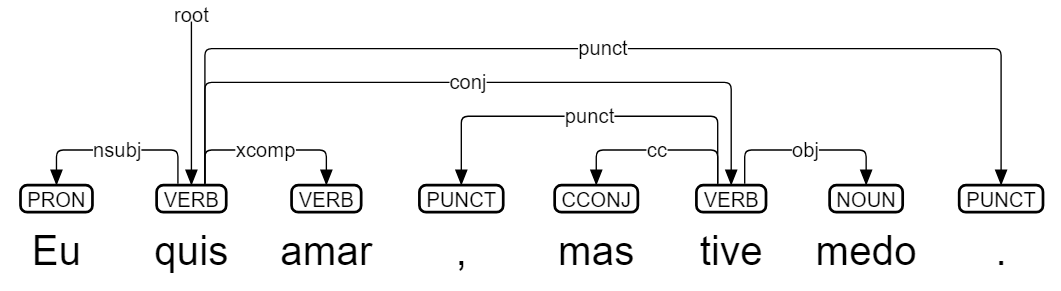
\includegraphics[scale=0.5]{images/lexicon_breakdown.png}
	\fautor
\end{figure}

A Análise de sentimentos emprega várias técnicas de \sigla{PLN}{Processamento de Linguagem Natural}, incluindo tokenização, lematização e remoção de palavras irrelevantes ou stop-words. A tokenização consiste em dividir o texto em palavras individuais ou "tokens". Já a lematização visa reduzir as palavras à sua forma base ou raiz, o que ajuda a consolidar diferentes formas da mesma palavra. Por sua vez, a remoção de palavras irrelevantes envolve a eliminação de termos comuns que geralmente não contribuem para o significado de uma frase, como "e", "o" e "em".Além dessas técnicas, a análise de sentimentos também se beneficia do uso de dicionários léxicos pré-existentes. Esses dicionários são valiosos recursos que contêm palavras associadas a valores de polaridade, indicando o sentimento geral de cada termo (positivo, negativo ou neutro).

No contexto da análise de sentimentos, existem vários dicionários léxicos relevantes disponíveis. Esse estudo comparou quatro repositórios bastante populares:

\begin{itemize}
	\item OpLexicon \cite{2011_Souza_IP}: É um dicionário léxico específico para o idioma português, com mais de 32.000 palavras, cada uma acompanhada de um valor de polaridade associado.
	\item SenticNet \cite{2016_Cambria_IP}: É dicionário léxico multilíngue que fornece valores de polaridade para palavras com base em sua semântica e psicologia.
	\item UniLex: Outro dicionário léxico multilíngue que oferece valores de polaridade para palavras com base em uma variedade de recursos linguísticos.
	\item WordNetAffectBR \cite{2008_Pasqualotti}: Esta é uma versão em português do WordNet-Affect, um dicionário léxico que atribui valores de polaridade às palavras com base em sua associação com diferentes emoções.
\end{itemize}

Ao utilizar esses dicionários léxicos, podemos comparar as palavras presentes no texto com as entradas nos dicionários para determinar a polaridade de cada uma. Isso nos possibilita obter uma compreensão mais abrangente dos sentimentos expressos no texto, contribuindo para uma análise de sentimentos mais precisa e eficaz. Esses dicionários são ferramentas valiosas no campo da análise de sentimentos, auxiliando na identificação e interpretação das emoções presentes nas palavras utilizadas. Além disso, com base nesses recursos, é possível automatizar e ampliar a análise de sentimentos em textos extensos, como avaliações de produtos, publicações em redes sociais e outros tipos de conteúdo textual.

Durante a comparação da polaridade da frase de teste com os dicionários léxicos, notou-se uma discrepância na normalização dos dicionários Unilex e WordNetAffectBR. Para este experimento, optamos por utilizar apenas o OpLexicon e o SenticNet, devido aos seus scores similares de polaridade e à presença de palavras exclusivas em cada um desses dicionários.

Além disso, realizamos um teste utilizando um \textit{subset} dos dados das postagens do Colab para adequação ao contexto. Durante esse teste, identificamos palavras relevantes que não estavam presentes nos dicionários léxicos originais. Adicionamos manualmente essas palavras ao conjunto de dicionários, atribuindo-lhes scores de -1 a 1 com base na polaridade observada nas postagens do Colab.

Em seguida, realizamos uma análise comparativa para avaliar a eficácia desses dicionários léxicos. Durante essa análise, calculamos a polaridade resultante para cada um dos dicionários, buscando identificar qual deles é mais eficaz na análise de sentimentos no contexto específico das postagens do Colab. Como resultado, obtivemos um amalgama dos dicionários OpLexicon e SenticNet, além do conjunto de palavras que foram adicionadas manualmente. Essas palavras foram normalizadas e incorporadas ao processo de análise.

A fim de enriquecer o conjunto de dados de treinamento e obter uma visão mais abrangente dos sentimentos expressos nas postagens do Colab, optamos por realizar uma amostragem aleatória do conjunto de dados original, adicionando 2000 eventos ao conjunto de treinamento. Essa abordagem nos permite incorporar uma maior diversidade de exemplos e aumentar a representatividade dos sentimentos presentes nas postagens. Ao selecionar aleatoriamente esses 2000 eventos, buscamos evitar qualquer viés de seleção que possa ocorrer ao escolher apenas os piores e melhores scores. Isso nos permite explorar uma variedade mais ampla de nuances de sentimentos que podem estar presentes no conjunto de dados geral. Além disso, ao combinar esses eventos adicionais com as postagens de scores mais altos e as postagens de scores mais baixos, temos um conjunto de dados de treinamento final composto por 3000 exemplos. Essa quantidade de dados é considerável e fornece uma base sólida para o treinamento do algoritmo de aprendizado de máquina.

Ao treinar o algoritmo com esse conjunto de dados, esperamos que ele aprenda a associar padrões linguísticos específicos a sentimentos positivos ou negativos, permitindo uma classificação automática mais precisa dos sentimentos expressos nas postagens do Colab. Essa abordagem baseada em aprendizado supervisionado nos permite utilizar os exemplos fornecidos no conjunto de dados de treinamento como referência para o desenvolvimento de um modelo que generalize e capture efetivamente os diferentes matizes de sentimentos presentes nas postagens.

\subsubsection*{Construção do modelo de classificação supervisionada de sentimentos}

Nessa seção, descrevemos a metodologia empregada para a análise de dados e a construção do modelo de aprendizado de máquina. Apresentamos no \autoref{codigo:sentiment_classifier} uma abordagem para realizar a análise de sentimento em postagens do Colab. Utilizamos técnicas de processamento de linguagem natural, vetorização de texto, além de algoritmos de aprendizado de máquina. Também incluímos visualizações por meio de WordCloud para identificar as palavras mais frequentes nas postagens.

O processo de análise de sentimento começa com o carregamento dos dados, que são pré-processados para normalizar as classificações de sentimento em 0 e 1. Em seguida, realizamos o pré-processamento do texto, que envolve a remoção de caracteres especiais, conversão para letras minúsculas, tokenização e aplicação de técnicas de stemização para reduzir as palavras às suas formas básicas \cite[]{2009_Bird_BOOK}.

Utilizamos a técnica de "bag-of-words" descrita em \citeonline{2013_Mikolov} com a biblioteca CountVectorizer para converter o texto em uma matriz numérica, onde cada coluna representa uma palavra e cada linha representa uma postagem. Com base nessa matriz, identificamos as palavras mais frequentes e as visualizamos em um gráfico de barras e na forma de uma nuvem de palavras.

\begin{figure}[!htb]
	\caption{Distribuição de palavras mais frequentes}
	\label{fig:wordcount}
	\centering
	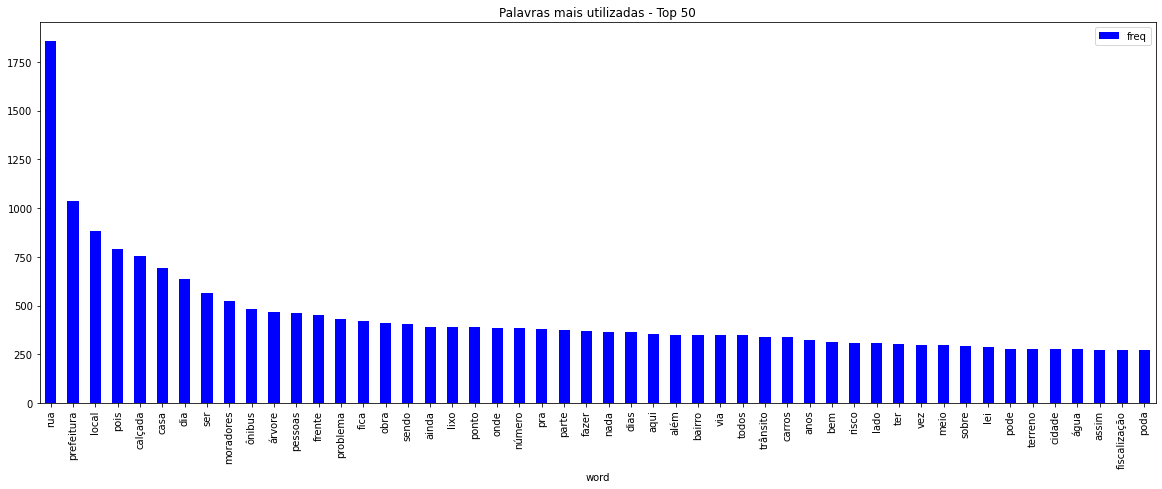
\includegraphics[scale=0.35]{images/wordcount.png}
	\fautor
\end{figure}

Realizamos uma análise exploratória dos dados para entender melhor as características das postagens. Isso incluiu a visualização da distribuição das palavras mais frequentes e a criação de nuvens de palavras para postagens positivas e negativas. Além disso, utilizamos a biblioteca Word2Vec para criar um modelo de palavras em vetores, que foi usado para visualizar as associações de palavras mais comuns.

\begin{figure}[!htb]
	\caption{Núvem de palavras mais utilizadas}
	\label{fig:wordcloud}
	\centering
	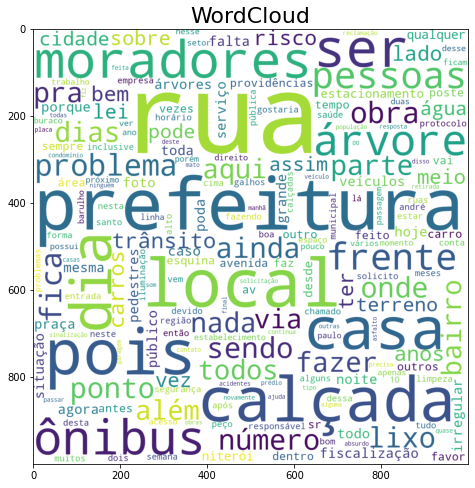
\includegraphics[scale=0.5]{images/wordcloud.png}
	\fautor
\end{figure}

\begin{figure}[htb]
	\centering
	\caption{Comparação de núvem de palavras mais usadas}\label{fig:lexicon_tagcloud}
	\begin{subfigure}[b]{0.317\textwidth}
		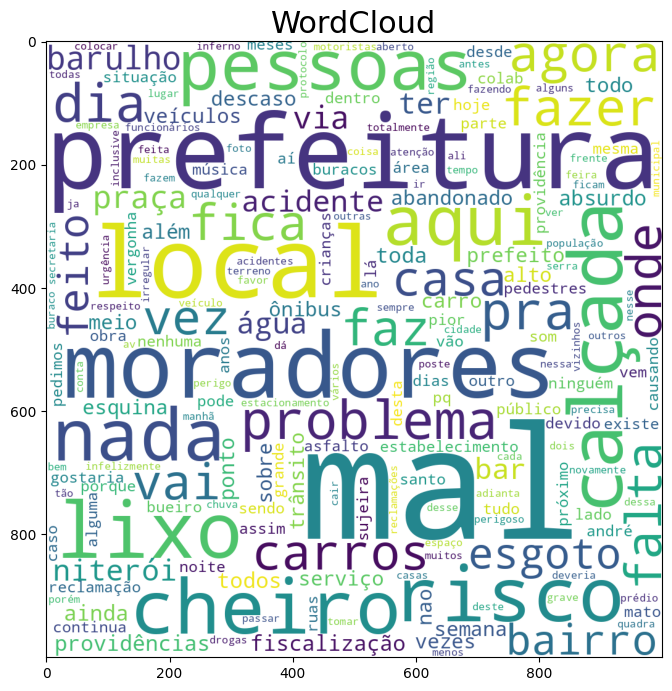
\includegraphics[width=\textwidth]{images/lexicon_worst_scores_tagcloud.png}
		\caption{Scores Negativos}
		\label{fig:tigre}
	\end{subfigure} ~ %add desired spacing between images, e. g. ~, \quad, \qquad, \hfill etc. %(or a blank line to force the subfigure onto a new line) 
	\begin{subfigure}[b]{0.317\textwidth}
		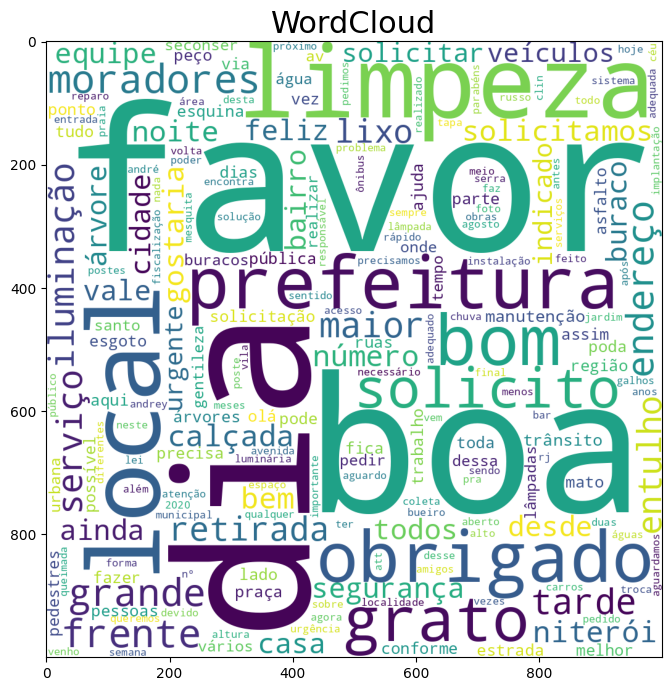
\includegraphics[width=\textwidth]{images/lexicon_best_scores_tagcloud.png}
		\caption{Scores Positivos} \label{fig:leao}
	\end{subfigure} ~ %add desired spacing between images, e. g. ~, \quad, \qquad, \hfill etc. %(or a blank line to force the subfigure onto a new line)
	\fautor
\end{figure}

Após a extração de recursos e análise exploratória, dividimos os dados em conjuntos de treinamento e validação. Em seguida, padronizamos os dados para garantir que todas as características tivessem a mesma escala \cite{2000_Jain}. Em seguida, realizamos o treinamento de diferentes modelos de classificação para tentar determinar o modelo mais apropriado para essa aplicação. A seguir, um breve resumo dos modelos utilizados:

\begin{itemize}
	\item \textbf{RandomForestClassifier}: Este algoritmo de aprendizado de máquina supervisionado utiliza o método de "bagging" e a técnica de árvores de decisão. Ele cria várias árvores de decisão e as combina para obter uma predição mais precisa e estável. O RandomForest é útil quando temos um grande conjunto de dados com muitas variáveis de entrada, e é eficaz para evitar o overfitting que pode ocorrer com árvores de decisão individuais \cite[5-32]{2001_Breiman}.
	\item \textbf{LogisticRegression}: A regressão logística é um algoritmo de aprendizado de máquina para classificação. No seu núcleo, é uma regressão, mas com uma função de ativação que transforma a saída em um valor entre 0 e 1. Este modelo é útil quando estamos lidando com problemas de classificação binária e queremos uma probabilidade associada a cada previsão \cite[215-242]{1958_Cox}.
	\item \textbf{DecisionTreeClassifier}: Este algoritmo de aprendizado supervisionado é usado principalmente para problemas de classificação. Ele funciona tanto para variáveis categóricas quanto contínuas. As árvores de decisão são úteis quando queremos um modelo que possa ser facilmente interpretado e explicado \cite[81-106]{1986_Quinlan}.
	\item \textbf{SVC (Support Vector Classifier)}: Este algoritmo de aprendizado de máquina é usado para classificação e regressão, mas é mais comumente usado para tarefas de classificação. O SVC é eficaz em espaços de alta dimensão e é útil quando o número de dimensões é maior do que o número de amostras \cite[273-297]{1995_Cortes}.
	\item \textbf{XGBClassifier (Extreme Gradient Boosting Classifier)}: Este algoritmo de aprendizado de máquina vai além do gradient boosting framework. O XGBoost é útil quando precisamos de um modelo que seja eficiente e tenha um alto desempenho, e é frequentemente usado em competições de ciência de dados devido à sua velocidade e precisão \cite[785-794]{2016_Chen_IP}.
\end{itemize}

Considerando o contexto de análise de sentimentos em busca de câmaras de eco, é crucial escolher um modelo de aprendizado de máquina que seja capaz de capturar com precisão as nuances e polaridades do sentimento expresso nos dados. Diversos estudos têm explorado diferentes modelos para análise de sentimento, cada um com suas próprias vantagens e limitações.

\citeonline{2016_Joshi} utilizaram RandomForest (RF) e Support Vector Machine (SVM) para classificar a polaridade de artigos de notícias financeiras e prever tendências de ações. Eles relataram que ambos os modelos tiveram bom desempenho, com uma precisão de mais de 80\%. Isso sugere que esses modelos podem ser eficazes na análise de sentimentos em câmaras de eco, especialmente quando os dados são ricos em recursos e a tarefa envolve a previsão de tendências com base na polaridade do sentimento.

Por outro lado, \citeonline{2017_Shen_IC} propuseram um modelo combinado de Convolutional Neural Networks (CNNs) e Bidirectional Long Short-Term Memory (BLSTM) para análise de sentimento de críticas de filmes. O modelo alcançou uma precisão de classificação de 89,7\%, que foi significativamente melhor do que a alcançada por CNN ou LSTM sozinhos. Este estudo sugere que modelos de redes neurais profundas, como CNN-BLSTM, podem ser particularmente úteis quando a análise de sentimento envolve a compreensão de sequências de texto complexas, como é frequentemente o caso em câmaras de eco.

\citeonline{2020_Han} propuseram uma função de kernel Fisher baseada em Probabilistic Latent Semantic Analysis para análise de sentimento usando SVM. Os autores relataram uma melhoria na classificação em comparação com os métodos tradicionais. Este estudo sugere que a incorporação de técnicas de análise semântica latente pode melhorar a eficácia dos modelos de análise de sentimento.

Finalmente, \citeonline{2020_Lin} propuseram um modelo de rede neural profunda aprimorado por comparação (Comparison Enhanced Bi-LSTM with Multi-Head Attention) para análise de sentimento. O modelo superou muitos modelos existentes em três conjuntos de dados de análise de sentimento. Este estudo sugere que modelos de atenção, que permitem que o modelo se concentre em partes relevantes do texto, podem ser particularmente eficazes na análise de sentimentos em câmaras de eco.

Em conclusão, embora não haja um único modelo "mais apropriado" para análise de sentimento em câmaras de eco, os estudos acima sugerem que modelos baseados em árvores, como RandomForest, modelos baseados em redes neurais, como CNN-BLSTM, e modelos que incorporam técnicas de análise semântica latente ou atenção podem ser particularmente eficazes.

A acurácia dos modelos foi avaliada utilizando o conjunto de validação e a pontuação F1 foi calculada para medir a precisão do modelo em ambas as classes. Além disso, as matrizes de confusão foram utilizadas para analisar o desempenho de cada modelo na classificação dos sentimentos, permitindo uma compreensão mais detalhada das previsões e erros cometidos.

No que diz respeito à modelagem de aprendizado de máquina, os resultados foram os seguintes:

\begin{itemize}
	\item \textbf{RandomForestClassifier:} O modelo RandomForestClassifier alcançou uma acurácia de treinamento de 0.996 e uma acurácia de validação de 0.172 na última execução em 19 de maio de 2022. Em uma execução anterior em 15 de maio de 2022, a acurácia de treinamento foi de 1.0 e a acurácia de validação foi de 0.14.
	\item \textbf{LogisticRegression:} O modelo LogisticRegression obteve uma acurácia de treinamento de 0.996 e uma acurácia de validação de 0.164 na última execução em 19 de maio de 2022. Em uma execução anterior em 15 de maio de 2022, a acurácia de treinamento foi de 1.0 e a acurácia de validação foi de 0.16.
	\item \textbf{DecisionTreeClassifier:} O modelo DecisionTreeClassifier alcançou uma acurácia de treinamento de 0.996 e uma acurácia de validação de 0.13 na última execução em 19 de maio de 2022. Em uma execução anterior em 15 de maio de 2022, a acurácia de treinamento foi de 1.0 e a acurácia de validação foi de 0.1.
	\item \textbf{SVC:} O modelo SVC obteve uma acurácia de treinamento de 0.395 e uma acurácia de validação de 0.098 na última execução em 19 de maio de 2022. Em uma execução anterior em 15 de maio de 2022, a acurácia de treinamento foi de 0.5906 e a acurácia de validação foi de 0.1.
	\item \textbf{XGBClassifier:} Na última execução em 15 de maio de 2022, o modelo XGBClassifier alcançou uma acurácia de treinamento de 0.3154 e uma acurácia de validação de 0.1.
\end{itemize}

Esses resultados indicam que o modelo RandomForestClassifier teve o melhor desempenho em termos de acurácia de treinamento, enquanto o modelo LogisticRegression teve a melhor acurácia de validação. No entanto, todos os modelos apresentaram uma grande diferença entre as acurácias de treinamento e validação, sugerindo que os modelos podem estar sofrendo de overfitting. Isso significa que os modelos estão se ajustando muito bem aos dados de treinamento, mas não estão generalizando bem para novos dados. Futuras iterações deste trabalho podem explorar técnicas para mitigar o overfitting, como a regularização ou o uso de mais dados de treinamento.

\subsection{Classificação de usuário por persona}

\subsubsection*{Geração de Dados de Treinamento para Classificação de Persona}

Os dados de treinamento para a classificação de persona foram gerados usando o ChatGPT. O ChatGPT foi treinado para gerar postagens de usuário que são representativas de "helpers" e "complainers". Estas postagens foram então usadas para treinar o modelo de classificação de persona. Eu vou melhorar essa seção depois.

\subsubsection*{Construção do modelo de classificação supervisionada por personas}

Utilizamos novamente o Python para classificar os usuários como "helpers" ou "complainers". O script utiliza o modelo de classificação de sentimento treinado para analisar as postagens dos usuários e determinar se eles são mais propensos a ajudar ou reclamar.

\section{Homofilia e Câmaras de Eco}

A homofilia, termo cunhado por Lazarsfeld e Merton em 1954, refere-se à tendência de indivíduos se associarem a outros que são semelhantes a eles em termos de características, interesses e opiniões. Esse fenômeno é amplamente estudado em diversas áreas, incluindo sociologia, psicologia e ciência das redes, e tem sido observado em várias configurações sociais, desde relacionamentos pessoais até interações online em redes sociais.

A homofilia pode estar intimamente relacionada às câmaras de eco, uma vez que a tendência de buscar semelhanças pode levar à formação de grupos com visões e perspectivas convergentes. Quando os indivíduos se associam principalmente a outros que compartilham suas opiniões, informações e conteúdos que são compartilhados dentro desses grupos tendem a reforçar e amplificar essas visões específicas. Isso cria um ambiente propício para o desenvolvimento de câmaras de eco, onde a diversidade de perspectivas é limitada e as ideias divergentes são escassas. A homofilia pode contribuir para a persistência das câmaras de eco ao restringir a exposição a opiniões contrárias e limitar a troca de informações entre diferentes grupos na rede. Essa dinâmica pode resultar em polarização, falta de entendimento mútuo e até mesmo no fortalecimento de crenças extremas.

Estudos têm destacado a relação entre homofilia e câmaras de eco em diferentes contextos, como a propagação de desinformação em redes sociais ou a formação de bolhas de opinião política. A presença de homofilia nas redes sociais pode contribuir para a criação de "filtros de informação" que reforçam as visões existentes e dificultam a exposição a diferentes perspectivas, aumentando assim a probabilidade de formação de câmaras de eco.

Ao entender o conceito de homofilia e sua relação com as câmaras de eco, podemos explorar métricas e técnicas para identificar e mitigar esses fenômenos nas redes sociais. A análise de métricas de homofilia pode fornecer insights sobre a estrutura das redes sociais e ajudar a compreender como as informações são disseminadas e as opiniões são formadas dentro desses contextos específicos. Essas descobertas podem ser fundamentais para desenvolver estratégias e intervenções que promovam uma maior diversidade de perspectivas, diálogo e compreensão mútua na era digital.

As métricas de homofilia geradas a partir deste experimento podem ajudar a detectar câmaras de eco em um grafo da rede do Colab. Câmaras de eco são fenômenos sociais onde as opiniões e informações são amplificadas ou reforçadas pela comunicação e repetição dentro de um sistema fechado e podem contribuir para a polarização social. Ao identificar e entender estas câmaras de eco, podemos desenvolver estratégias para promover a diversidade de opiniões e a comunicação aberta.

\section{Classificação de personas em Modelagem Baseada em Agentes}

A Modelagem Baseada em Agentes (MBA) é uma técnica computacional que tem ganhado interesse em diversas áreas de pesquisa, devido à sua capacidade de simular a interação de agentes autônomos e observar os resultados emergentes dessas interações. A MBA é particularmente útil para estudar sistemas complexos, onde o comportamento global do sistema não pode ser facilmente deduzido a partir do comportamento individual dos agentes.

Agora, consideremos as personas "helpers" e "complainers" em redes sociais. Estas personas, embora não sejam explicitamente mencionadas por Atiqi, podem ser consideradas como agentes dentro da estrutura de MBA. Os "helpers" podem ser vistos como agentes que buscam transmitir mensagens positivas e úteis, enquanto os "complainers" tendem a transmitir mensagens negativas ou críticas. A interação entre essas duas personas pode levar a diferentes dinâmicas de rede e padrões de comunicação. Por exemplo, se os "helpers" são mais influentes ou numerosos, eles podem criar um ambiente mais positivo e cooperativo na rede social. Por outro lado, se os "complainers" são mais influentes ou numerosos, eles podem criar um ambiente mais negativo e crítico.

Além disso, a presença de bots também pode influenciar a dinâmica entre "helpers" e "complainers". Por exemplo, bots programados para agir como "helpers" podem aumentar a positividade e a cooperação na rede, enquanto bots programados para agir como "complainers" podem aumentar a negatividade e a crítica. Portanto, a abordagem de MBA usada por Atiqi se torna uma ferramenta útil para estudar a interação entre "helpers" e "complainers" em redes sociais e entender como essas interações podem influenciar a dinâmica da rede e a formação da opinião pública.